

\begin{frame}

Economic theory: A higher minimum wage reduces employment \vskip .2in \pause
Data
\begin{itemize}
\item Apr 1 1991: Federal minimum wage rises to \$4.25
\item Apr 1 1992: New Jersey minimum wage rises to \$5.05
\end{itemize} \vskip .2in \pause
\bgray{Theoretical Estimand}: Effect of the law on employment in NJ \pause
$$\underbrace{Y_\text{NJ,After}^1}_\text{Observed}\quad  - \underbrace{Y_\text{NJ,After}^0}_\text{Counterfactual}$$
where $Y$ is employment, \\ \pause
superscript $A = 1$ is \$5.05 minimum wage, and\\ pause
superscript $A = 0$ is \$4.25 minimum wage

\end{frame}




\begin{frame}
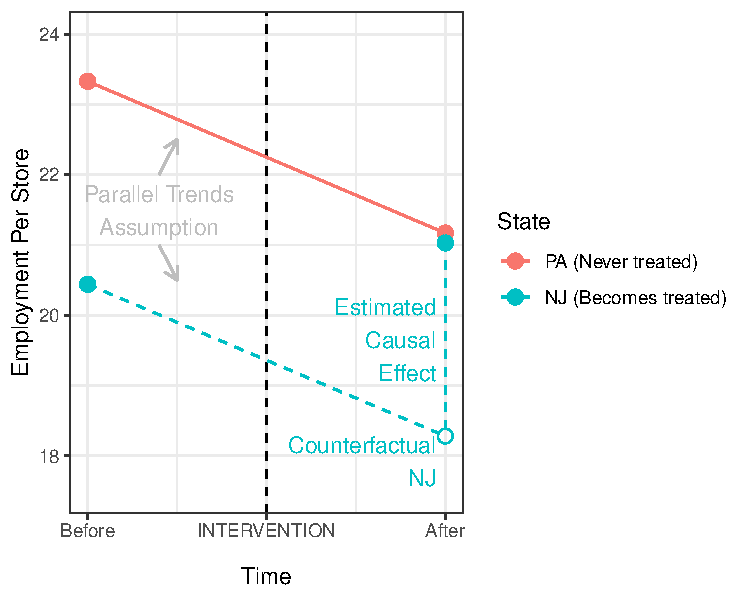
\includegraphics[width = .3\textwidth]{figures/ck_slide5.pdf} \vskip .1in \pause
\bgray{Parallel trends assumption:} \pause If no law had taken effect, then \pause
$$\overbrace{Y_\text{NJ,After}^0  - Y_\text{NJ,Before}^0}^\text{the trend in NJ} \overbrace{=}^\text{would equal} \overbrace{Y_\text{PA,After}^0 - Y_\text{PA,Before}^0}^\text{the trend in PA} $$ \pause
Rearranging yields a formula for the counterfactual outcome \pause
$$
\underbrace{Y_\text{NJ,After}^0}_\text{Counterfactual} \overbrace{=}^\text{By Assumption} \pause \underbrace{Y_\text{NJ,Before}^0 + Y_\text{PA,After}^0 - Y_\text{PA,Before}^0}_\text{Factual}
$$ \pause
$$\text{Effect in NJ} = \underbrace{Y_\text{NJ,After}^1}_\text{Observed}\quad  - \underbrace{Y_\text{NJ,After}^0}_\text{Estimated by Above}$$
\end{frame}

\begin{frame}{Can we test the parallel trends assumption?}

\onslide<2->{\bred{No.}}
\only<1>{$$\overbrace{Y_\text{NJ,After}^0  - Y_\text{NJ,Before}^0}^\text{Assumption: The trend in NJ} \overbrace{=}^\text{would equal} \overbrace{Y_\text{PA,After}^0 - Y_\text{PA,Before}^0}^\text{the trend in PA} $$}
\only<2->{$$\overbrace{\begin{red}\underbrace{Y_\text{NJ,After}^0}_\text{Not Observable}\end{red}  - Y_\text{NJ,Before}^0}^\text{Assumption: The trend in NJ} \overbrace{=}^\text{would equal} \overbrace{Y_\text{PA,After}^0 - Y_\text{PA,Before}^0}^\text{the trend in PA} $$} \vskip .2in
\onslide<3->{You can make it credible by looking at many pre-treatment periods}

\end{frame}

\begin{frame}[t]{DID would be very credible}
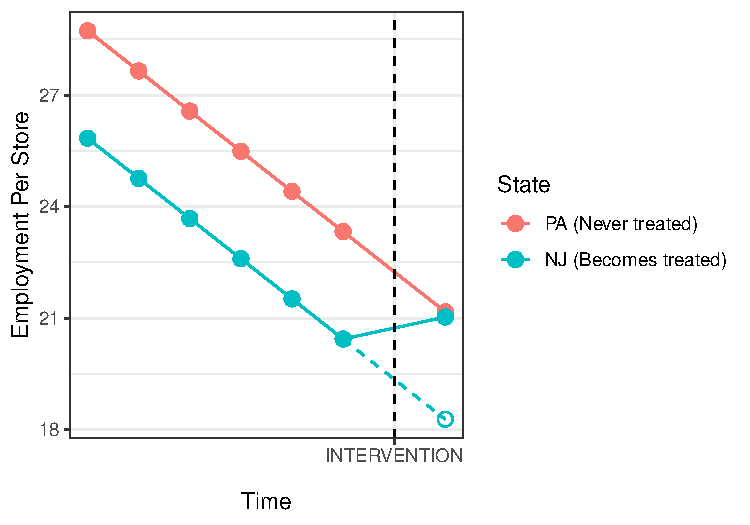
\includegraphics[width = \textwidth]{figures/parallel_trends_credible.pdf}
\end{frame}

\begin{frame}[t]{DID would be very doubtful}
\includegraphics<1>[width = \textwidth]{figures/parallel_trends_doubtful.pdf}
\includegraphics<2>[width = \textwidth]{figures/parallel_trends_doubtful_2.pdf}
\end{frame}


Agricultural center is

Is there any agriculture extension center in this commune?

Tap water is answer = 1, 2, or 3


What is the main source of drinking /cooking water for most people in this commune
during the [.season.]?
Indoor private piped water 1
Outdoor private piped water 2
Public piped water 3
Well water 4
Well with protection walls 5
Well without protection walls 6
Stream water with protection 7
Stream water without protection 8
Rainwater 9
Bottled water 10
Water brought by pedicab 11
Tank water 12
river lake pond………… 13
other (specify_________________) 14